\chapter{Introduction}
\label{ch:intro}

The nature of dark matter (DM) remains one of the major unsolved problems in physics. Originally inferred through its gravitational influence on galaxies and clusters, a rich body of evidence has accumulated over the last four decades firmly establishing its existence. All of the evidence, however, comes from inferring dark matter's presence solely through its gravitational effects. Much else about it remains an open question: Does dark matter consist  of a fundamental particle? If so, what is its mass? Could there be an entire dark sector, akin to the Standard Model (SM)? How does dark matter interact with the SM? The quest to answer these questions represents a huge collective effort that draws from a rich body of theoretical and experimental work, as well as major input from the computational and numerical side. We are currently at the dawn of a data-driven era in astrophysics and cosmology---a large number of ongoing and forthcoming experiments, both in the lab and in the sky, combined with an increasingly open approach to data availability offer great potential in elucidating the nature of dark matter. 

Dark matter plays a central role in many subfields of particle physics, astrophysics and cosmology. Understanding its nature and interactions would have far reaching consequences, as there is no concrete explanation within the framework of the Standard Model of particle physics. It would represent a paradigm shift in those fields and provide major insights into fundamental physics beyond the Standard Model, as well as elucidate the evolution of our Universe and the formation of structures within it. 

% While there exists a proliferation of ideas regarding the particle nature of dark matter, the dominant paradigm over the last three decades has been that of the Weakly Interacting Massive Particle (WIMP), which posits dark matter to consist of a particle with weak-scale interactions with the Standard Model, produced through thermal freeze-out in the early universe. This framework dovetails well, for example, with supersymmetric extensions to the Standard Model where candidates for dark matter can emerge naturally. After briefly describing alternative explanations, in this thesis I will focus exclusively on WIMP searches. I will also focus exclusively on astrophysical searches for WIMPs.

This introduction is organized as follows. In Sec.~\ref{sec:evidence}, I will summarize the large body of evidence pointing to the existence of dark matter. In Sec.~\ref{sec:particledm}, I will describe possible explanations for the particle nature of dark matter and various detection paradigms, focusing on DM thermally produced in the early Universe and specifically Weakly Interacting Massive Particles (WIMPs). Section~\ref{sec:astrodm} will focus on the effort to detect and characterize WIMPs through their astrophysical signature, in particular using gamma-ray data. I will briefly summarize the theoretical and experimental tools available to us in these searches. Finally, in Sec.~\ref{sec:summary}, I will describe the organization of the rest of this thesis. % Wherever possible, I will touch upon the historical developments that have paved the way for our current state of understanding of dark matter and our efforts to look for it.

\section{Evidence for Dark Matter}
\label{sec:evidence}

Although the study of dark matter had its inception and development in the 20th century, the interplay between theory and observation in making the unknown knowable goes back much earlier. For example, the Aristotelian view of an immutable Universe with the Earth as its center offered a clean framework that did not call for additional invisible matter or celestial objects, and was the orthodox viewpoint until Renaissance astronomers conclusively refuted it with observations. Galileo, in the face of significant resistance from the Catholic Church, arguably played the largest role in this and discovered much that was previous unknowable -- including understanding the make-up of the Milky Way as consisting of individual stars rather than diffuse clouds, and observing Saturn's rings and Jupiter's four largest moons. These observations are very much in the spirit of modern dark matter searches -- demonstrating that the Universe can contain invisible forms of matter, and that scientific inquiry and technological developments can play a big role in revealing them to us.

% \subsection{Dynamical Evidence}

Evidence for some yet-unknown form of matter started piling up in the early 19th century. Lord Kelvin introduced the idea of applying the ``theory of gases'' to the Milky Way, describing stars as gas particles acting under the influence of gravity and in the process wondered whether a large number of stars may actually be dark bodies. In 1922, Dutch astronomer Jacobus Kapteyn wrote down for the first time a predictive model for the distribution of matter in the Milky Way, describing the stars as particles in a virialized system~\cite{1922ApJ....55..302K}. Kapteyn used this method to obtain the local matter density in term of the the observed stellar mass, diving out the gravitational mass by the number of stars observed. Kapteyn's student Jan Oort~\cite{1932BAN.....6..249O} as well as others during this time~\cite{1922MNRAS..82..122J} were able to derive estimates for the density of matter in the local neighborhood, usually claiming that an excess above the observed luminous mass, if any, could be accounted for by the extrapolation of the stellar luminosity function down to very faint stars.

In 1933, Swiss-American astronomer Fritz Zwicky studied redshift data for galaxy clusters collected by Hubble and Humason~\cite{1931ApJ....74...43H}, noticing large velocity dispersions in eight galaxies within the Coma cluster and applying the virial theorem to estimate its mass~\cite{1933AcHPh...6..110Z}. Zwicky predicted the dispersion by using the number of observed galaxies, average mass of a galaxy and its extent, finding a value closer to 80 km\,s$^{-1}$. This was in stark conflict with the observed line-of-sight velocity dispersion of 1000 km\,s$^{-1}$. Although Zwicky's work made use of an estimate of the Hubble constant that was a factor of $\sim$8 too big compared to the current accepted value, the large discrepancy between the observed and expected values pointed to the existence of unaccounted-for matter in the Coma system. Zwicky himself concluded that ``If this would be confirmed, we would get the surprising result that dark matter is present in much greater amount than luminous matter''. An analysis of the Virgo cluster by Sinclair Smith in 1936 again pointed to a very high mass-to-light ratio in that system. In either case, the astronomers put forward potential explanations in terms of ``clouds of low-luminosity internebular material''~\cite{1937ApJ....86..217Z}.

Although this represented a conundrum, there was widespread consensus that more information would be needed to understand what was going on. Historically, velocity rotation curves---the circular velocity profiles of stars in a galaxy as a function of the distance from the galactic center---did the most to convince the scientific community to the existence of large amounts of non-luminous matter in galaxies. The basic idea here is as follows. Standard Newtonian theory dictates that the circular velocity of stars is given by $v_c(r) = \sqrt{GM/r}$, where $r$ is the radial distance, $M$ the enclosed mass and $G$ the universal gravitational constant. In the region beyond the galactic disk (defining the observed extent of the galaxy), we expect the enclosed mass to be constant, and Gauss' law dictates that the circular velocity fall as $v_c \propto r^{-1/2}$. The detection of the 21-cm emission line in 1950s heralded a new era in radio astronomy and enabled the accurate measurement of rotation curves. Measurements by Vera Rubin and others throughout the 1970s, starting with those of the nearby galaxies M31 and M33 and indeed our own Milky Way, pointed to the approximate flattening out of rotation curves at larger radii contrary to above expectation~\cite{1970ApJ...159..379R,1973A&A....26..483R}, and implications for the missing mass problem were realized soon after~\cite{1974Natur.250..309E,1974ApJ...193L...1O}. This implied that the mass continues to increase as $M \propto r$, pointing to the existence of additional unobserved `dark' mass beyond the visible component. From this, the density of dark matter can be inferred to roughly scale as $\rho(r) \propto 1/r^2$. A large number of observations on galactic and cluster scales since then have strengthened the case for the existence of halos of dark matter extending far beyond the visible extent of these objects. The left panel of Fig.~\ref{fig:evidence} shows the measured rotation curves for the Milky Way compiled in Ref.~\cite{2009PASJ...61..227S} compared with theoretical expectations from disk- and bulge-like components (green and red lines, respectively) inferred from baryonic matter, as well as an additional dark matter component from a spherical, isothermal dark matter halo (yellow line). It can clearly be seen that the additional DM halo component is required to match the observed rotation curves. The component descriptions are provided in Ref.~\cite{2009PASJ...61..227S}.

Cosmology provides substantial evidence supporting the existence of dark matter in our Universe. $\Lambda$CDM, often referred to as the standard model of cosmology, is associated with the presence of dark energy ($\Lambda$) and cold dark matter (CDM), is able to account for a plethora of cosmological observations, including the existence and structure of the cosmic microwave background (CMB) radiation, large-scale structure distribution of matter, accelerating expansion of the Universe and relic elemental abundances~\cite{Dodelson:1282338,Kolb:1990vq}. The CMB, which represents the imprint of photons that decoupled from the baryon-photon fluid about 370,000 years ago and have been free-streaming ever since, by itself provides irrefutable evidence for (non-baryonic) dark matter. The primary relevant observable is the angular scale of inhomogeneities in the temperature distribution of the CMB -- the $TT$ angular power spectrum. The spectrum largely consists of a set of peaks, each peak giving us an angular scale with a particularly significant contributions to the temperature fluctuations. The leading physical effect behind these are acoustic oscillations in the baryon-photon fluid during photon decoupling. Early on, photons and baryons were electromagnetically coupled, and non-baryonic dark matter was responsible for generating gravitational potential wells that could pull in the baryon-photon fluid. The photon pressure acting against these wells gave rise to a tower of modes, imprinted in the CMB as the acoustic peaks. While the detailed physics is somewhat nuanced\footnote{See Wayne Hu's CMB tutorials for an excellent introduction: \url{http://background.uchicago.edu/index.html}.}, the relative heights of these peaks can provide information about the energy content of our Universe, including the relative composition of baryonic and non-baryonic (dark) matter. Very heuristically, the position of the first peak provides information about the curvature of the universe (and hence how much total ``stuff'' there is in it), while the second peaks tells us how much of the matter is baryonic (ordinary matter). The third peak and its relative height can shed insights into the abundance of non-baryonic dark matter. Historically, the WMAP satellite, while not able to fully resolve the third peak, was already able to conclusively say that dark matter makes up the majority of the matter budget in the Universe, finding the baryon density $\Omega_b h^2=0.02264\pm0.00050$ and cold dark matter density $\Omega_c h^2=0.1138\pm0.0045$~\cite{2013ApJS..208...19H}. Since then, \emph{Planck} has been able to precisely measure eight peaks of the $TT$ spectrum, finding $\Omega_b h^2= 0.02225\pm0.00016$ and $\Omega_c h^2=0.1198\pm0.0015$ from the $TT$, $TE$ and $EE$ spectra. The right panel of Fig.~\ref{fig:evidence} shows the \emph{Planck} $TT$ spectrum~\cite{Ade:2015xua} along with the best-fit theoretical predictions (blue line), as well as predictions for a slightly altered cosmology $\Omega_b h^2= 0.042$ and $\Omega_c h^2=0.10$ with a reduced dark matter density, where striking differences from the measured spectrum can be seen.

The above is by no means exhaustive -- many other observations over a large range of scales provide evidence for the existence of dark matter, including observations of the distribution of galaxies on large scales, weak and strong lensing of background galaxies by foreground structure, and observations of merging clusters.

\begin{figure}[htbp] 
\hspace{-0.9 cm} 
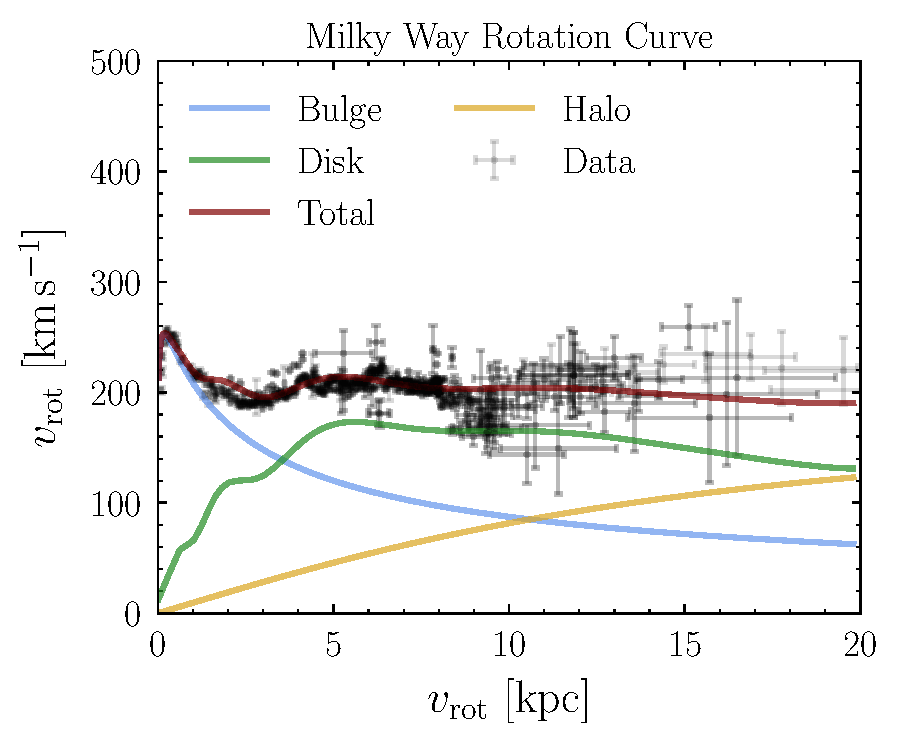
\includegraphics[width=0.5185\textwidth]{ch-intro/rotcurves.pdf}
 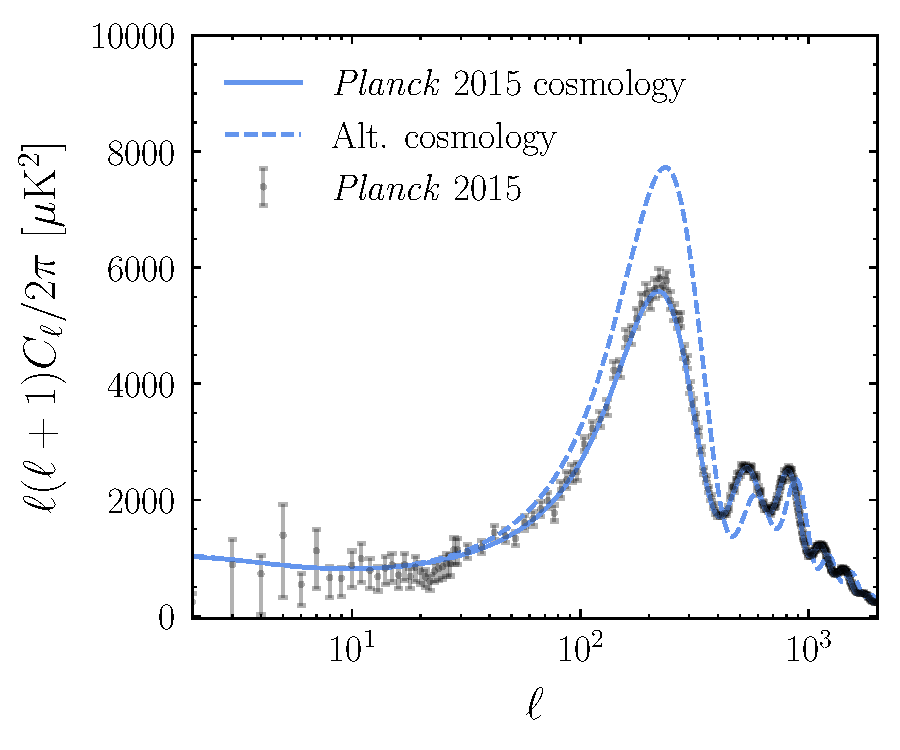
\includegraphics[width=0.528\textwidth]{ch-intro/cells.pdf}  
\caption{(Left) The measured rotation curves for the Milky Way compiled in Ref.~\cite{2009PASJ...61..227S}, and theoretical expectations from disk- and bulge-like components (green and red lines, respectively) inferred from baryonic matter~\cite{2009PASJ...61..227S}, as well as an additional dark matter component from a spherical, isothermal halo (yellow line). (Right) The \emph{Planck} $TT$ spectrum~\cite{Ade:2015xua} along with the best-fit theoretical predictions (blue line, computed with \texttt{CAMB}~\cite{Lewis:1999bs}), as well as predictions for a slightly altered cosmology with $\sim$10\% less non-baryonic (dark) matter where striking differences from the observed spectrum can be seen.}  
\label{fig:evidence}
\end{figure}


\section{(Particle) Nature of Dark Matter}
\label{sec:particledm}

Although the existence of dark matter is incontrovertible, its nature largely remains a mystery. These days, it is often implicitly assumed that when people are talking about detecting dark matter, say at a Xenon direct detection experiment or in gamma ray data, that this refers to a dark matter \emph{particle}. As touched upon above, this has by no means always been the case -- early usage and references to dark matter usually referred to the existence of generic dark objects that would be too faint to be observed, such as dim stars or internebular material. The transition in usage from an adjective to a noun was a result of sociological changes within the particle physics and astrophysics communities, bringing the two closer after the missing mass problem had been firmly accepted in the 1970s. All evidence amassed since then is consistent with dark matter being a fundamental particle, or even the existence of an entire dark sector consisting of many particles with a rich set of properties and interactions.

Within the Standard Model, neutrinos---by virtue of being stable (or very long-lived), electrically neutral particles that do not interacting strongly---contain some of the essential attributes for a particle dark matter candidate, and were discussed in this context early on. Cosmological effects of neutrinos were discussed throughout the 1960s and 1970s, pioneered by the work of Zeldovich and others~\cite{Gershtein:1966gg,PhysRevLett.29.669}, and their implication for the missing mass observed on (super-)galactic scales was discussed in the the late 1970s~\cite{PhysRevLett.39.165,1978ApJ...223.1015G}. Early simulations during the 1980s eventually showed that hot (relativistic) and cold (non-relativistic) particle dark matter would lead to very different outcomes for structure formation, leading to formation and collapse of larger structures---``top-down''---in the former case and a hierarchical ``bottom-up'' structure formation, where overdensities seed larger structures, in the latter. Neutrinos, by virtue of being very light thermal relics, would be extremely relativistic during structure formation and, combined with these simulations, early surveys of the local Universe were able to quickly discount them as dark matter candidates~\cite{1983ApJ...274L...1W}. Nevertheless, along the way neutrinos served as gateway particles in understanding the implications of potential new particles to observations on galactic, cluster and cosmological scales.

With no reason to be confined to the Standard Model, supersymmetry (SUSY) posits that nature may contain a spacetime symmetry relating bosons and fermions, requiring that for ever boson a fermion with the same quantum numbers must exist (and vice versa)~\cite{Wess:1974tw,PhysRevLett.48.223}. This leads to the prediction of several new electrically neutral particles that are uncharged under the strong force. If some of these were stable, they could have played an important role in the history of our Universe and could conceivably make up (some portion of) the dark matter~\cite{Jungman:1995df}. Supersymmetry took its modern form with a paper by Dimopolous and Georgi, who introduced the Minimal Supersymmetric Standard Model (MSSM)~\cite{Dimopoulos:1981zb}. Here, superpartners of the $Z$ boson, photon and two Higgses mix to form four particles, known today as neutralinos. Neutralinos have arguably been the most-discussed dark matter candidate~\cite{Bertone:2004pz}, in part because supersymmetry--with its ability to enable gauge coupling unification and solve the electroweak hierarchy problem---is motivated in its own right independent of the dark matter problem, and the existence of a viable DM candidate is often seen as a desirable bonus.

Besides SUSY-motivated particles such as neutralinos, there is no shortage of viable particle DM candidates today, including but not limited to axions~\cite{PhysRevLett.40.223,Peccei:1977hh}, sterile neutrinos~\cite{Abazajian:2001nj,Seljak:2006qw}, and light (sub-GeV) dark matter~\cite{Feng:2008ya,Lin:2011gj}. The most general constraints on the properties of particle DM, \emph{e.g.} its mass, are relatively mild. In particular, observations constrain $m_\text{boson} \gtrsim 10^{-22}$\,eV for bosons~\cite{Zhang:2017chj} (with ultralight scalar ``fuzzy'' DM a viable candidate at the lowest end~\cite{Hui:2016ltb}) , and $m_\text{fermion} \gtrsim 0.7$\,keV for fermions~\cite{Horiuchi:2013noa}. This is obtained from observations of DM halos around dwarf galaxies, imposing the requirement for particles to occupy a minimum phase-space volume according to the uncertainty principle for bosons and the Pauli exclusion principle for fermions. An upper limit of $\sim$10$^{48}$\,GeV comes from searches for microlensing signatures of MACHOS (Massive Astrophysical Compact Halo Objects) in our Galaxy~\cite{Griest:2013aaa}.

\subsection{Thermal Dark Matter and WIMPs}

There are several general and striking features pertaining to dark matter particles in thermal equilibrium with the Standard Model in the early Universe. Warmer (lower mass) thermal relics strongly suppress structure formation at smaller scales~\cite{Bringmann:2006mu}, and the DM mass is accordingly constrained to be $\gtrsim 3.3$\,keV from an analysis of the power spectrum of the Lyman-$\alpha$ flux~\cite{Viel:2013apy}. Unitarity arguments place an upper bound of $\lesssim340$\,TeV on the mass of a stable particle that was once in thermal equilibrium with the SM~\cite{Griest:1989wd}, although this is model-dependent and assumes that there are no states heavier than the DM. Additionally, a weak-scale self-annihilation cross section of $\langle\sigma v\rangle\sim 3\times10^{-26}$\,cm$^3$\,s$^{-1}$ and GeV-TeV particle masses can reproduce the observed DM density through freeze-out in the early Universe (see Refs.~\cite{1991NuPhB.360..145G,1996PhR...267..195J,Lisanti:2016jxe} for further details). This fact holds for a large variety of electroweak-scale DM candidates, and combined with the theoretical arguments for the existence of new physics at electroweak scales these particles---known as Weakly Interacting Massive Particles (WIMPs)---have been the dominant particle dark matter paradigm over the last three decade and have motivated an extensive search program. 

Searches for WIMPs are generally organized into three categories depending on the experimental detection paradigm. Direct detection, which looks for the energy deposited when dark matter particles recoil against nuclei through the process $\text{SM}\,\chi\rightarrow\text{SM}\,\chi$, where $\chi$ is a DM particle. While the flux of WIMPs through a terrestrial detector can be large, the expected deposited energies and interaction rates would be very small, requiring large amounts of target material and exquisite control over backgrounds~\cite{Lisanti:2016jxe}. Direct detection experiments have been able to set very strong limits on WIMP scenarios~\cite{Aprile:2018dbl,Agnes:2018ves} and have been able to exclude several attractive baseline models~\cite{Escudero:2016gzx}. The second class of searches involves production of WIMPs at particle colliders like the Large Hadron Collider (LHC) through the process $\mathrm{SM}\,\mathrm{SM}\rightarrow\chi\,\chi$, usually in association with additional visible particles emitted by initial or intermediate SM particles that can used to detect the event along with the missing energy characterizing the WIMP. Dedicated collider searches can also target specific scenarios, such as neutralino production~\cite{Patrignani:2016xqp}. See Ref.~\cite{Kahlhoefer:2017dnp} for a recent review of collider searches for dark matter.

The final strategy and the focus of this thesis is indirect detection, which looks for the annihilation of DM particles into SM particles through the process $\chi\,\chi\rightarrow\mathrm{SM}\,\mathrm{SM}$ by looking for its signature in astrophysical data. The nature of the SM particles depends on the specific DM model and interaction properties considered. The basic idea behind indirect detection is that annihilation processes will be taking place at higher rates in regions of the Universe that have more dark matter, leading to an excess in production of SM particles from those regions. These would then cascade on to photons, electrons, positrons, (anti)protons and neutrinos, some of which could eventually reach us and be detected with appropriate telescopes. %In the next section, I will introduce some of the challenges associated with indirect detection searches and tools required to perform them. 

It is worth noting that the WIMP scenario, while well-motivated, relies on several assumptions that can easily be relaxed~\cite{PhysRevD.43.3191}. The possibility of the DM relic density set by annihilations into heavier states (``Forbidden'' DM)~\cite{DAgnolo:2015ujb,PhysRevD.43.3191} or $3\rightarrow2$ annihilations of Strongly Interacting Massive Particles (SIMPs)~\cite{Hochberg:2014dra,Hochberg:2014kqa} are representative examples where relatively small modifications to the WIMP paradigm can lead to very different ranges of allowed masses and cross sections.

\section{Indirect Detection of Annihilating Dark Matter}
\label{sec:astrodm}

As noted above, for generic thermal WIMP scenarios where the DM can self-annihilate, its late-time abundance is set by the coupling of the DM particle to the Standard Model. The expected self-annihilation cross section in this case is entirely predictive and we would expect an electroweak-scale cross section around $\langle\sigma v\rangle\sim 3\times10^{-26}$\,cm$^3$\,s$^{-1}$, and a particle mass of $m_\chi\sim\mathcal O($GeV-TeV). DM particles in this mass range annihilating to SM particles would cascade on to photons falling dominantly in the gamma-ray range. This regime is well-probed by today's gamma-ray telescopes, including the \emph{Fermi} Large Area Telescope (\emph{Fermi}-LAT)~\cite{Atwood:2009ez}, data from which will be used in the analyses presented in this thesis. Terrestrial observatories such as HAWC~\cite{Abeysekara:2014ffg}, H.E.S.S.~\cite{Abdallah:2018qtu}, MAGIC~\cite{Ahnen:2017pqx}, VERITAS~\cite{Archambault:2017wyh} and the upcoming CTA~\cite{Doro:2012xx} can typically achieve better sensitivity at higher photon energies (and correspondingly higher DM masses $m_\chi\gtrsim 100$\,GeV) due to their much larger effective area. Observation of cosmic ray spectra (specifically positrons and antiprotons) from experiments like AMS-02 can be sensitive probes of DM annihilation in certain cases (\emph{e.g.}, leptonic final states)~\cite{Aguilar:2014mma,Bergstrom:2013jra}, although there are large systematic uncertainties inherited from the uncertainties on Galactic propagation of charged cosmic rays. See Ref.~\cite{Slatyer:2017sev} for a comprehensive recent review of indirect dark matter searches.   % In this section, I will describe the ingredients necessary to calculate the expected DM annihilation flux and discuss common astrophysical search targets. 

\subsection{Tools for Indirect Detection}
\label{subsec:tools}

A major challenge for indirect detection searches is to calculate the dark matter annihilation flux expected from a given astrophysical target or source population. The basic prescription for doing so is as follows. If the DM particle number density at angular coordinates $\psi$ (describing the angle away from the Galactic plane) located at a line-of-sight distance $l$ from us is $n[r(l,\psi)]$ and the self-annihilation cross section is $\langle\sigma v\rangle$, the annihilation rate per particle is given by
\begin{equation}
n[r(l,\psi)]\langle\sigma v\rangle = \frac{\rho[r(l,\psi)]}{m_\chi}\langle\sigma v\rangle,
\end{equation}
where $\rho[r(l,\psi)]$ is the DM density and $m_\chi$ its particle mass. The total annihilation rate in a volume element $dV = l^2\,dl\,d\Omega$ is given by convolving this quantity by the number of particles in the volume:
\begin{equation}
\frac{\rho[r(l,\psi)]}{m_\chi}\langle\sigma v\rangle \frac{\rho[r(l,\psi)]}{2m_\chi}dV.
\end{equation}
where the factor of $2$ in the denominator is to avoid double counting since two particles are involved in the annihilation process. The total observed annihilation flux is obtained by integrating along the line of sight and over a given angular extent:
\begin{equation}
\frac{d\Phi}{dE}(E,\Psi) = \frac{1}{4\pi}\int\,d\Omega\,dl\,\rho[r(l,\psi)]^2\frac{\langle\sigma v\rangle}{2m_\chi^2}\frac{dN}{dE}
\end{equation}
where the photon energy spectrum $dN/dE$ gives the number of photons produced per annihilation for a given 2-body final state, and can be obtained with parton shower tools like \texttt{Pythia8}~\cite{Sjostrand:2007gs} or from tabulated values for certain specific cases~\cite{Cirelli:2010xx}. The annihilation cross section can often be factorized out of the integral, but this is not possible if the cross section has a strong velocity-dependence, e.g. in $p$-wave annihilation scenarios\footnote{See Ref.~\cite{Slatyer:2017sev} and references therein for further details on photon spectra and velocity-suppressed annihilations.}. %All astrophysical information is contained in the so-called $J$-factor, which is the line-of-sight integral along a given direction of the squared dark matter density. 
In the simplest cases where this is possible, the annihilation flux factorizes as
\begin{equation}
\frac{d\Phi}{dE}(E,\Psi) = \underbrace{\frac{\langle\sigma v\rangle}{8\pi m_\chi^2}\frac{dN}{dE}}_{d\Phi_\mathrm{PP}/dE}\underbrace{\int\,d\Omega\,dl\,\rho[r(l,\psi)]^2}_J
\end{equation}
where $d\Phi_\mathrm{PP}/dE$ encapsulates the particle physics assumptions, and $J\equiv\int\,d\Omega\,dl\,\rho[r(l,\psi)]^2$ is the so-called $J$-factor and captures the astrophysical dependence of the flux. Objects with higher $J$-factors over some localized region typically make for more interesting indirect detection targets. However, a high $J$-factor by itself does not a good annihilation target guarantee -- this must additionally be balanced with how well the systematic uncertainties on both the properties of the potential signal as well as astrophysical backgrounds and Galactic foregrounds can be accounted for and controlled.

\subsection{Sources of Gamma Rays from Annihilating Dark Matter}
\label{subsec:dmsources}

An important challenge in indirect detection is to accurately characterize the DM signal and associated uncertainties. This often involves astrophysical input as well as input from observations at other wavelengths and $N$-body simulations. Given the typically sizable systematic uncertainties, it is crucial to have the ability to probe the same DM parameter space with multiple complementary targets. The following sources are generally used as targets in annihilation searches:  %Roughly, the $J$-factor scales as $\sim(\int\rho^2\,dV)/d^2$, where $\rho$ is the DM density distribution and $d$ the distance of the object from us. The following objects are generally considered as targets in DM annihilation searches: 
\begin{itemize}
\item \emph{Milky Way dwarf galaxies}: Being dark matter dominated and having relatively low expected astrophysical backgrounds, dwarf spheroidal satellite galaxies (dSphs) of the Milky Way have traditionally been considered excellent targets for DM annihilation searches. There have been about 45 dSphs candidates discovered recently by surveys like SDSS and DES, and searches for gamma-ray emission from these have been able to place strong constraints on annihilation scenarios, constraining thermal WIMPs below $\lesssim 70$~GeV at 95\% confidence level for the case of annihilation into  the $b\bar b$ final state~\cite{Fermi-LAT:2016uux,Ackermann:2015zua}. The relevant $J$-factors are far from well-characterized, however -- assumptions about \emph{e.g.}, the dSph halo shape~\cite{Geringer-Sameth:2014qqa,Sanders:2016eie} and stellar membership criteria used to infer the halo properties~\cite{2016MNRAS.462..223B,Geringer-Sameth:2014yza} can lead to significant uncertainties on the predicted annihilation signal. Figure~\ref{fig:sources} (top right) shows a map of the inferred $J$-factors of dSphs considered in Ref.~\cite{Fermi-LAT:2016uux}. As in that study, the dSphs are assumed to be point-like since the shape of the corresponding DM halos is not very well constrained.
\item \emph{The Milky Way halo}: Our own Galaxy is the brightest source of DM emission in the sky. Figure~\ref{fig:sources} (top left) shows the expected annihilation $J$-factor for the smooth component of our Galactic halo (see caption for further details). 

Searches in the inner Galaxy, where the signal is expected to be the brightest, have yielded an excess emission whose spatial and spectral properties can be consistent with those of a DM annihilation signal (\emph{e.g.}, a $\sim$40\,GeV WIMP annihilating to $b\bar b$ with an approximately thermal cross section), often called the Galactic center excess~\cite{Daylan:2014rsa,Goodenough:2009gk,Hooper:2010mq,Calore:2014xka,Gordon:2013vta}. This region of the sky is however complicated by the presence of substantial and difficult-to-characterize Galactic foregrounds, which complicates the interpretation of any signal and/or constraint from this region. Indeed, recent results based on analyzing the statistics of photons in the region~\cite{Lee:2015fea,Bartels:2015aea} (see also Ch.~\ref{ch:nptfit}) indicate that the excess is more consistent with emission from an unresolved population of point sources rather than a dark matter signal, which is expected to be more diffuse in nature.

Another class of searches focus on looking for DM emission from the Milky Way halo over larger regions of the sky at higher Galactic latitudes, where the signal is still appreciable but Galactic foregrounds are much lower. These studies necessitate being able to accurately characterize the Galactic foreground emission over larger regions of the sky, and a careful consideration of these effect yields stringent limits, excluding thermal WIMPs at masses below $\lesssim 70$~GeV at 95\% confidence level for the case of annihilation into $b\bar b$~\cite{Chang:2018bpt}.

\item \emph{Galactic substructure}: Hierarchical bottom-up structure formation necessitates the existence of substructure within galaxies, and subhalos have the potential to be attractive DM annihilation targets. Unlike classical and ultrafaint dwarf galaxies mentioned above, low-mass subhalos with virial mass $M_\mathrm{vir}\lesssim 10^8$\,M$_\odot$ would be mostly dark with highly suppressed stellar activity~\cite{2017MNRAS.467.2019R,Fitts:2016usl}, which makes it difficult to localize them and look for their gamma-ray emission. Figure~\ref{fig:sources} (bottom left) shows a simulated realization of $J$-factors for Galactic substructure (subhalos) following the prescription in~\cite{Hutten:2016jko}.

Traditional searches rely on attempting to characterize the emission from unassociated gamma-ray sources detected by \emph{Fermi} as potentially coming from DM annihilation in individual subhalos, and comparing these observations to expectations from $N$-body simulations~\cite{Bertoni:2015mla,Calore:2016ogv,Hooper:2016cld,Schoonenberg:2016aml}. The bright source in the top right corner of the substructure map in Fig.~\ref{fig:sources}, for example, would likely show up as a resolved unassociated source in \emph{Fermi} point source catalogs such as 3FGL.

An orthogonal approach is to study the statistics of photons associated with DM annihilation from a population of dim subhalos. These subhalos may not be detectable individually, but their collective emission could show up as a heightened level of ``clumpiness'' in the photon map. Statistical methods described in Chs.~\ref{ch:nptfit} and ~\ref{ch:igrb} of this thesis can be used to look for this structure in gamma-ray data, and this application is currently a topic of ongoing study.

\item \emph{Extragalactic galaxies and clusters}: Searches for DM annihilation in extragalactic targets have traditionally been complicated by the difficulty in characterizing the DM properties of extragalactic halos and the presence of potentially significant astrophysical emission. Searches for emission from individual, nearby clusters~\cite{Ackermann:2015fdi}, the integrated, isotropic emission from background halos~\cite{Ackermann:2015tah,Ajello:2015mfa,Cholis:2013ena,DiMauro:2015tfa}, and cross-correlation of gamma rays with local catalogs of galaxies and large-scale structure~\cite{Ando:2013xwa,Ando:2014aoa,Ando:2016ang,Cuoco:2015rfa,Regis:2015zka,Xia:2015wka} have yielded constraints on DM annihilation. These searches typically do not attain sensitivity to thermal WIMPs for realistic astrophysical assumptions, however. Chapter~\ref{ch:groups_sim} of this thesis focuses on developing methods to systematically characterize the dark matter emission from a large number of nearby extragalactic galaxies and clusters along with the associated uncertainties~\cite{Lisanti:2017qoz}. Figure~\ref{fig:sources} (bottom right) shows the extragalactic $J$-factor map derived using this prescription and the group catalogs from Refs.~\cite{Tully:2015opa} and~\cite{2017ApJ...843...16K}. Chapter~\ref{ch:groups_data} presents a search for gamma-ray emission using this map, placing stringent limits on annihilating DM and excluding thermal WIMPs at masses below $\lesssim 40$~GeV at 95\% confidence level for the case of annihilation into $b\bar b$~\cite{Lisanti:2017qlb}.
\end{itemize}

\begin{figure}[htbp] 
\centering
 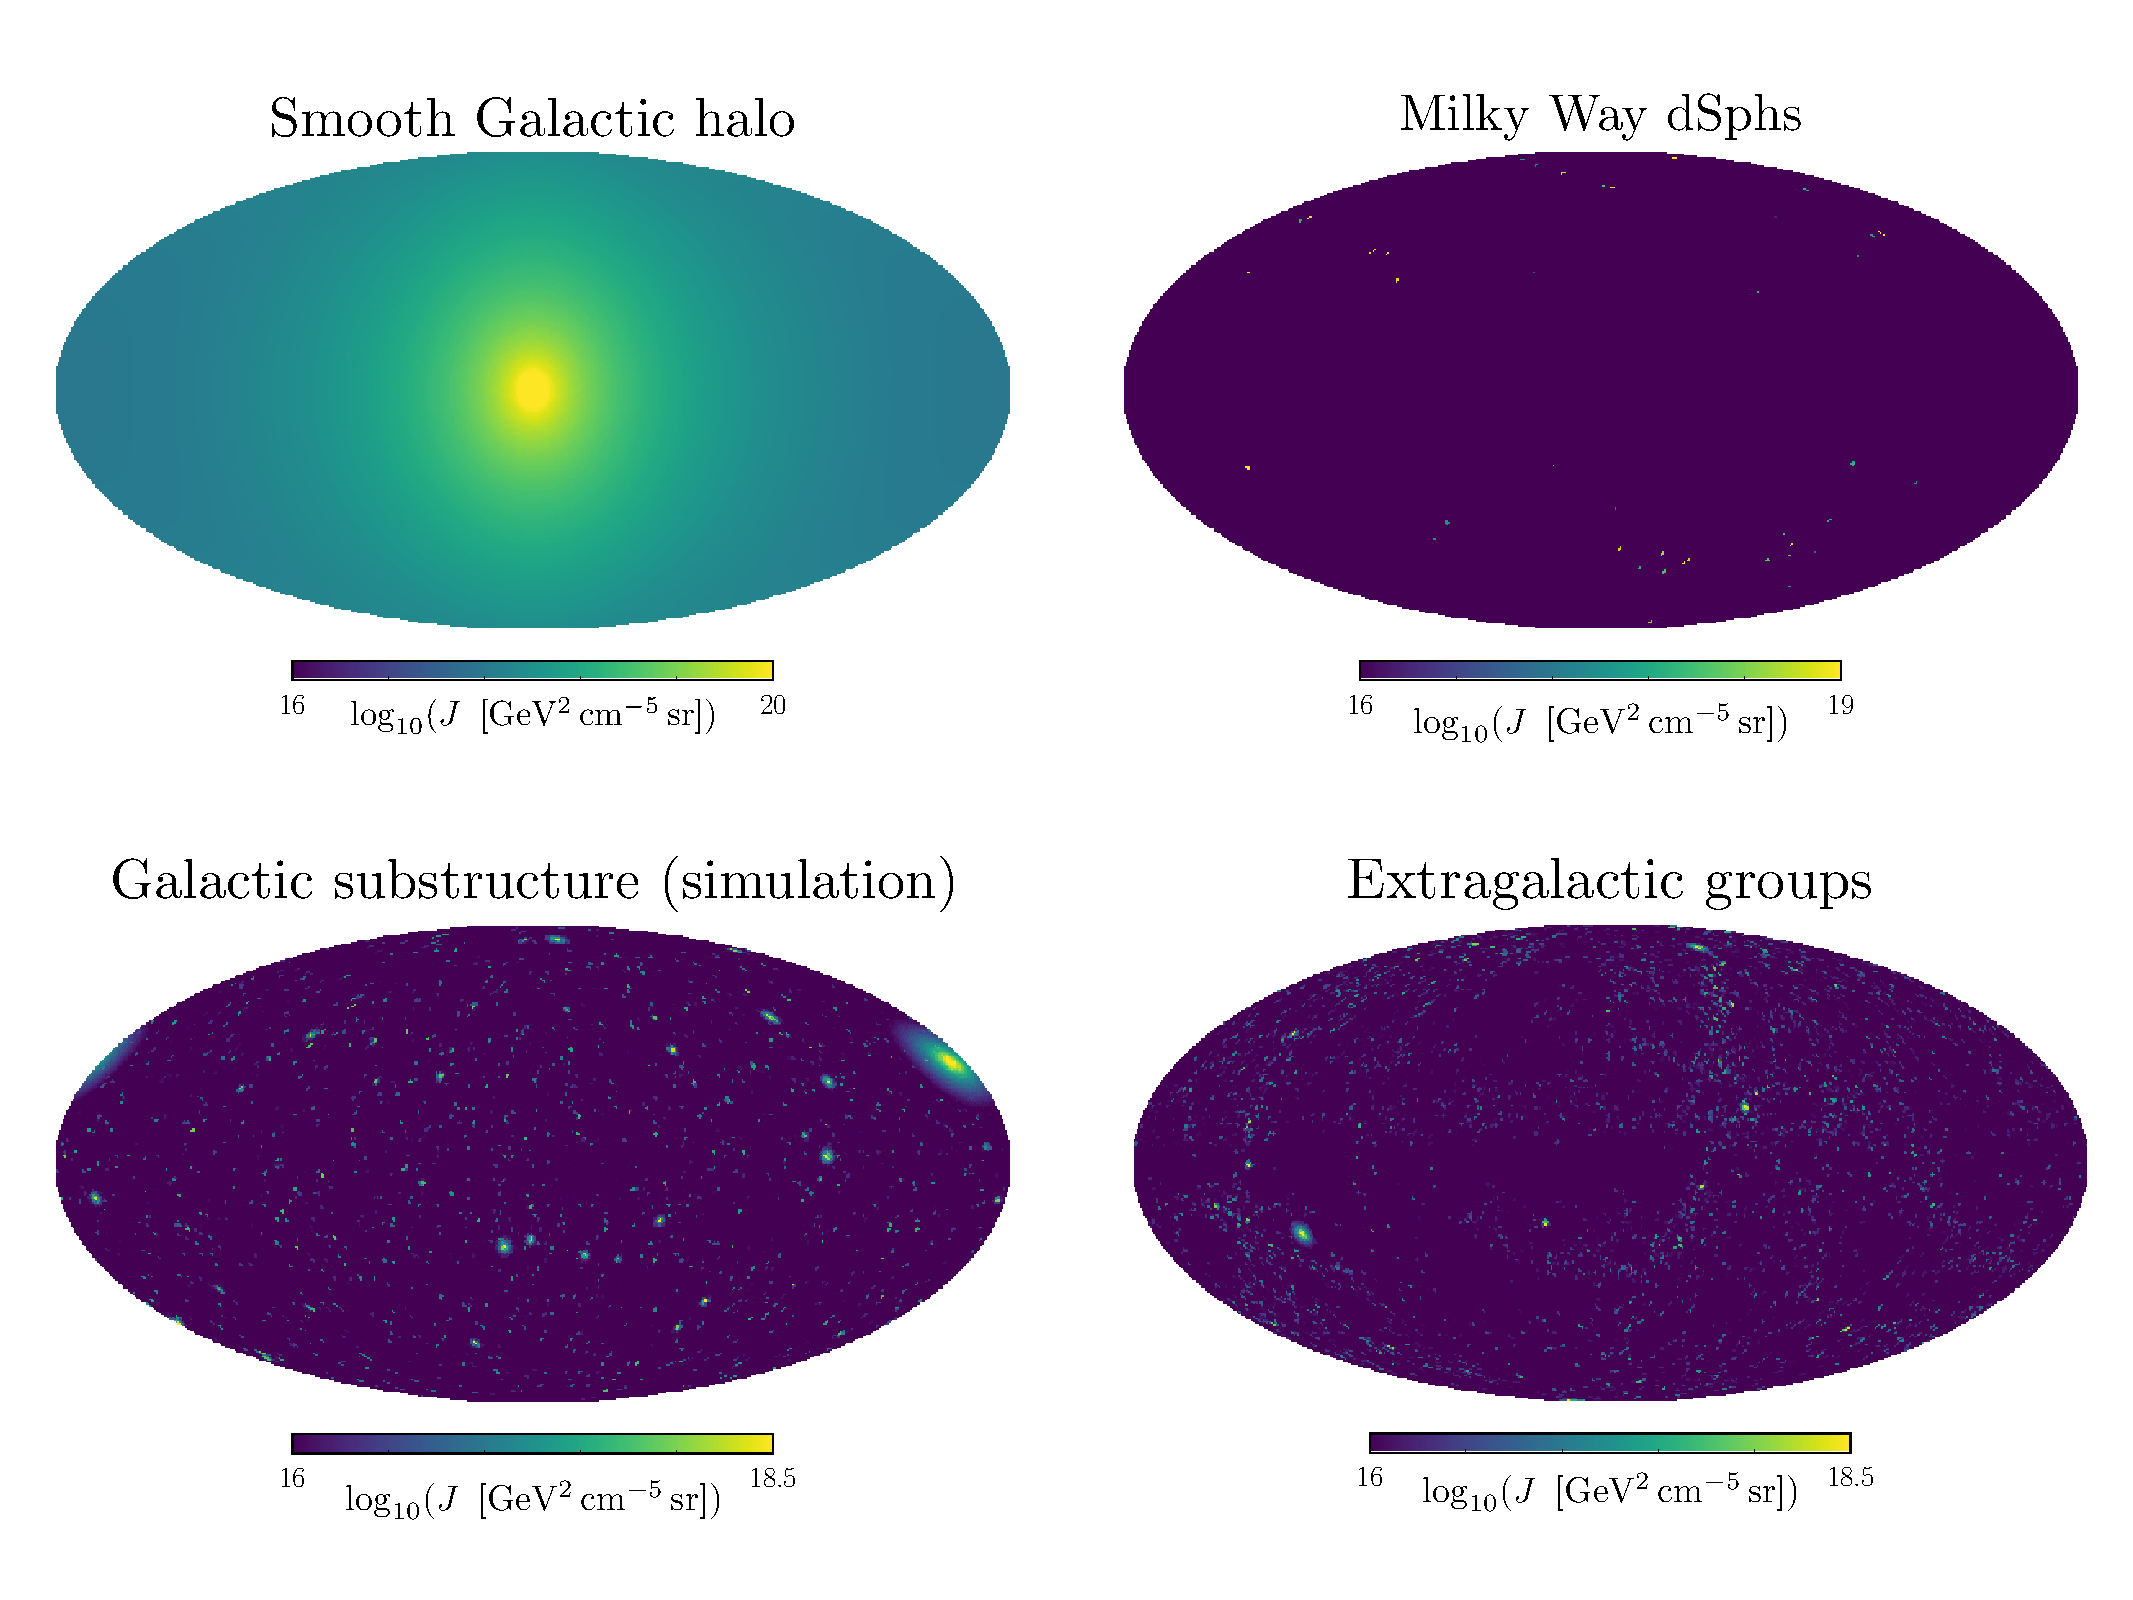
\includegraphics[width=1.0\textwidth]{ch-intro/jfactors.pdf}
\caption{Maps of annihilation $J$-factors showing targets commonly considered in gamma-ray searches. \textbf{(Top left)} The smooth Galactic halo, assuming a canonical NFW dark matter profile $\rho_\text{NFW}(r)=\frac{\rho_{s}}{r/r_{s}\,(1+r/r_{s})^{2}}$, where $r_s=17$ kpc is the Milky Way scale radius and $\rho_s$ is the normalization chosen to reproduce the local DM density $\rho_\text{NFW}(r_\odot) = 0.4$ GeV$\,$cm$^{-3}$~\cite{2015ApJ...814...13M,Sivertsson:2017rkp} at the Solar radius $r_\odot = 8$~kpc~\cite{Read:2014qva}. \textbf{(Top right)} Milky Way dwarf spheroidal galaxies (dSphs) as considered in Ref.~\cite{Fermi-LAT:2016uux}. Following that study, the dSphs are assumed to be point-like sources since the properties of the corresponding DM halos are not currently well constrained. \textbf{(Bottom left)} A simulated realization of $J$-factors for Galactic substructure (subhalos) following the prescription in~\cite{Hutten:2016jko}. Subhalos are spatially distributed according to the results of the Aquarius simulation~\cite{Springel:2008cc} and a halo mass distribution of $dN/dm\propto m^{-1.9}$ is assumed. The concentration-mass parameterization from Ref.~\cite{Sanchez-Conde:2013yxa} is used and DM in the subhalos is assumed to be NFW-distributed. The number of subhalos is calibrated to give 300 objects between $10^8$-$10^{10}$\,M$_\odot$. The bright source in the top right corner of the map would likely show up as a resolved unassociated source in \emph{Fermi} point source catalogs such as 3FGL~\cite{Bertoni:2015mla}. \textbf{(Bottom right)} $J$-factors of extragalactic groups derived using properties compiled in the group catalogs of Refs.~\cite{Tully:2015opa} and~\cite{2017ApJ...843...16K} and the prescription presented in Chs.~\ref{ch:groups_sim} and \ref{ch:groups_data}.}  
\label{fig:sources}
\end{figure}


\subsection{Template Methods for Gamma-Ray Searches}
\label{subsec:statmethods}

Data from gamma-ray detectors such as \emph{Fermi}-LAT is typically a series of maps, representing the number of photons binned spatially as well as in energy. Figure~\ref{fig:data} illustrates a subset of this data. The challenge lies in disentangling a potential DM signal, which could represent emission from large-scale structures such as the smooth Galactic halo as well as point/extended sources like dwarf galaxies, from astrophysical backgrounds. The most common technique for understanding the contribution of various potential contributions to gamma-ray data is Poissonian template fitting, which we briefly describe here; a detailed description will be given in Ch.~\ref{ch:groups_sim}. 

\begin{figure}[htbp] 
\centering
 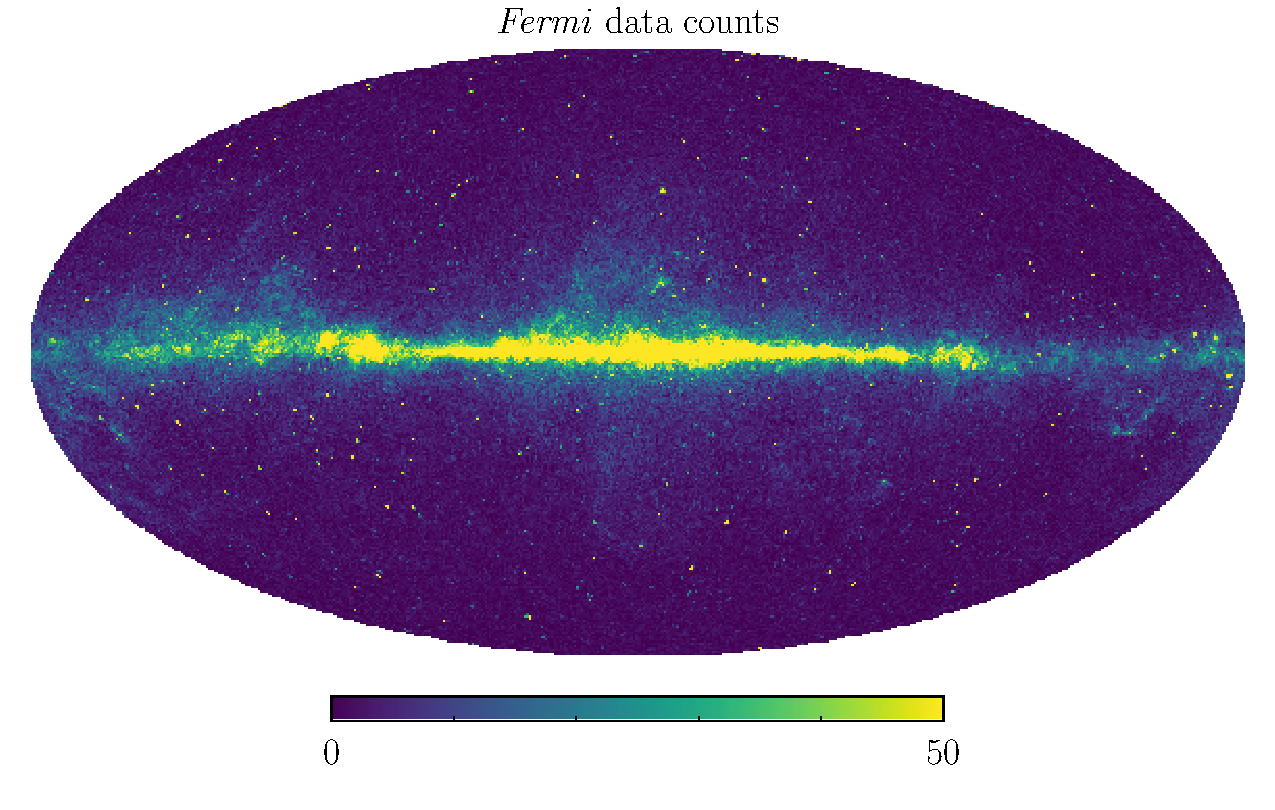
\includegraphics[width=0.8\textwidth]{ch-intro/data.pdf}
\caption{A subset of the photons collected by \emph{Fermi}-LAT between August 4, 2008 and July 7, 2016. The data corresponds to photons in the energy range 2-20 GeV. Additionally, the top quartile of the UltracleanVeto event class (PSF3) as ranked by angular resolution is considered and the recommended quality cuts are applied (see Ch.~\ref{ch:groups_sim} for further details).}  
\label{fig:data}
\end{figure}

A template is a spatial map which describes the modeled contribution of a particular source of class of sources to the data. This could represented, for example, the expected emission from the diffuse Galactic foreground emission, or emission due to resolved astrophysical point sources. Figure~\ref{fig:templates} shows some templates commonly used in \emph{Fermi} gamma-ray analyses (see caption for descriptions). Templates for DM emission can be constructed as described in Secs.~\ref{subsec:tools} and \ref{subsec:dmsources}. Restricting ourselves to a single energy bin for now and representing the value of a given template $i$ in pixel $p$ by $T_i^p$, the total expected counts in pixel $p$ is given by 
\begin{equation}
\mu^p(\boldsymbol \theta) = \sum_i A_i\,T_i^p,
\end{equation}
where $\boldsymbol \theta$ represents the signal and background model parameters ${A_i}$, which in this case are the corresponding template normalizations. The key observation is that the pixelized data is expected to be a Poisson realization of the sum of modeled components. In this case, the likelihood function for the parameters $\boldsymbol \theta$ given the data is a product of the Poisson probabilities associated with the observed counts $n^{p}$ in each pixel of the region-of-interest:
\begin{equation}
\mathcal{L}(d | {\boldsymbol \theta}) = \prod_p \frac{\mu^{p}({\boldsymbol \theta})^{n^{p}} e^{-\mu^{p}({\boldsymbol \theta})}}{n^{p}!}\,.
\label{eq:pi}
\end{equation}
With the likelihood in hand, we can understand the contribution of various components using conventional inference methods, \emph{e.g.} obtaining the parameter posteriors within a Bayesian framework or building up a likelihood surface for certain parameters of interest using frequentist profile likelihood techniques. The latter is more commonly used in DM searches -- typically, we are more interested in the parameters associated with the DM model (\emph{e.g.} its particle mass $m_\chi$ and annihilation cross section $\langle\sigma v\rangle$, which can be mapped on to a particular normalization of the DM template) than those corresponding to the astrophysical backgrounds. A likelihood surface $\mathcal{L}(d|\mathcal M, m_\chi, \langle\sigma v\rangle)$ for the signal parameters corresponding to a given DM model $\mathcal M$ can be obtained by maximizing the likelihood for the background parameters at each signal parameter point, profiling them out. When analyzing several energy bins and/or stacking multiple sources (\emph{e.g.} several extragalactic halos), the total likelihood can be obtained as the product of the individual likelihoods.

\begin{figure}[htbp] 
\centering
 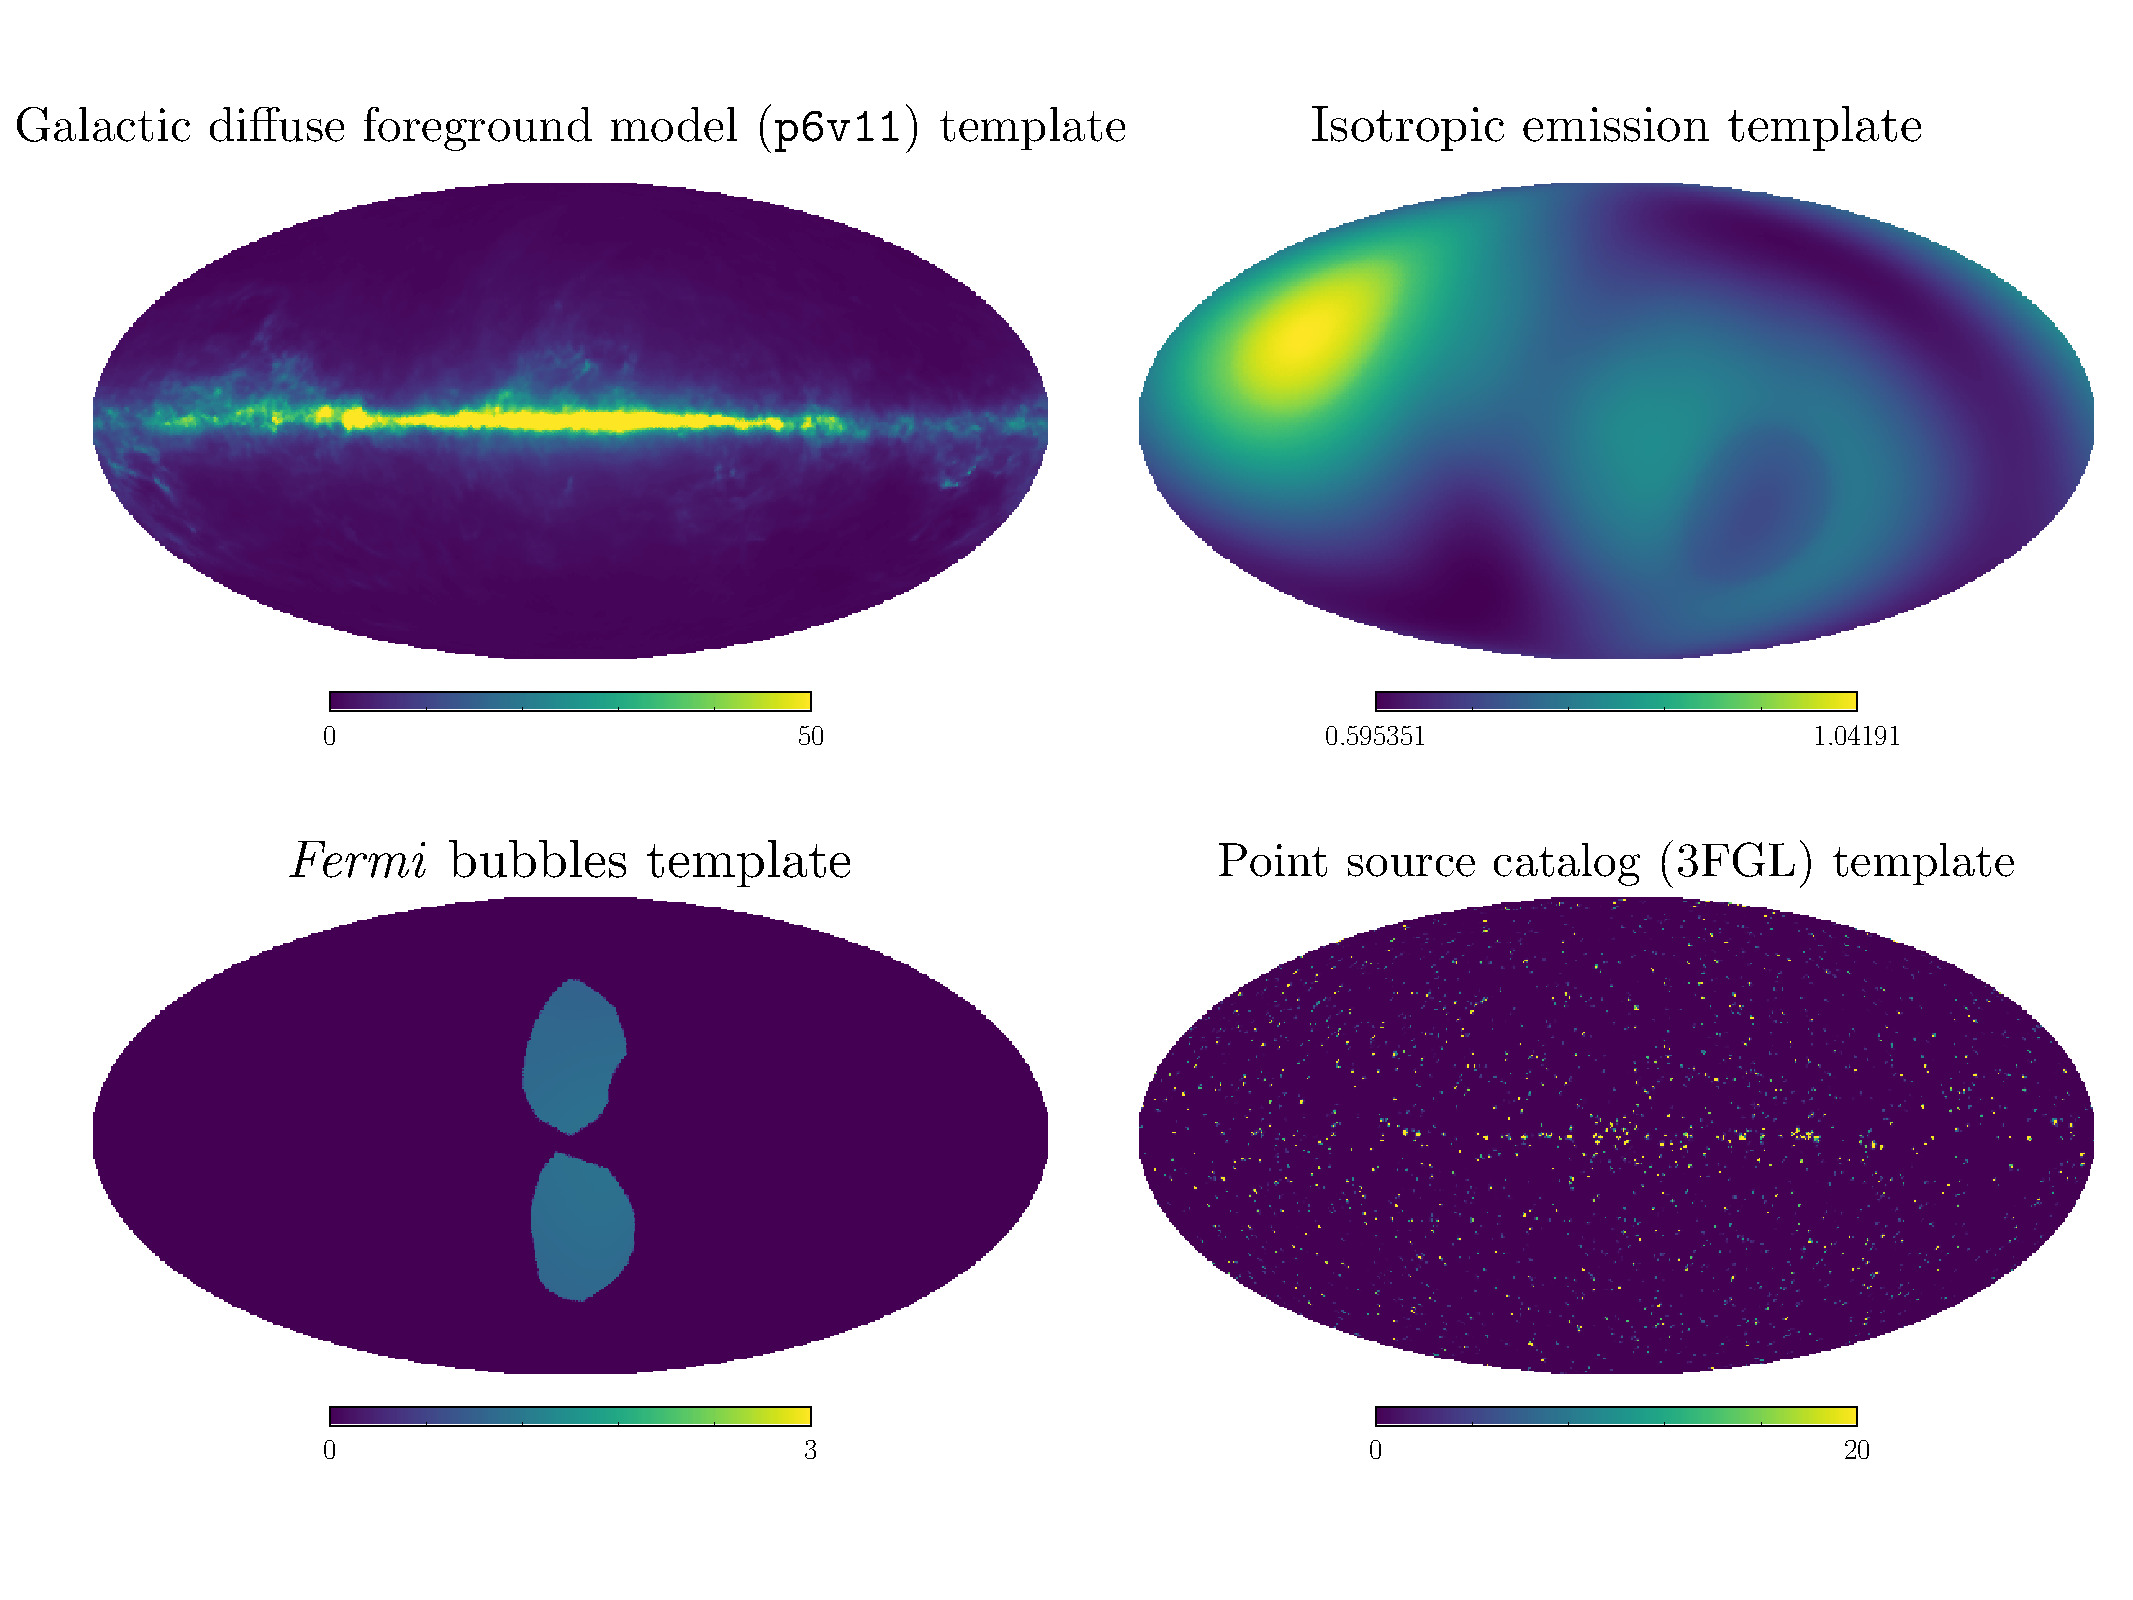
\includegraphics[width=1.0\textwidth]{ch-intro/templates.pdf}
\caption{Representative templates commonly considered in \emph{Fermi}-LAT gamma-ray analyses. The normalizations of the templates are such that these represent the best fit to the data shown in Fig.~\ref{fig:data}. \textbf{(Top left)} Template for the Galactic diffuse foreground emission, as modeled by the  {\it Fermi} \texttt{p6v11} model. \textbf{(Top right)} Isotropic template, intended to account for emission from unresolved extragalactic point sources. This template is not perfectly uniform due to the non-uniform exposure of the LAT instrument. \textbf{(Bottom left)} Template for the \emph{Fermi} bubbles, two lobe-like structures likely of astrophysical origin~\cite{Su:2010qj,Fermi-LAT:2014sfa}. \textbf{(Bottom right)} Template for resolve point sources as compiled in the \emph{Fermi} 3FGL catalog~\cite{Acero:2015hja}.}  
\label{fig:templates}
\end{figure}


For inferring dark matter properties, a log-likelihood ratio test statistic (TS) can be defined for a given mass $m_\chi$ against the null hypothesis ($\langle\sigma v\rangle=0$) as
\begin{equation}\begin{aligned}
{\rm TS}(\mathcal{M}, \{ \langle\sigma v\rangle, m_\chi\}) \equiv 2 &\left[ \log \mathcal{L}(d | \mathcal{M}, \{\langle\sigma v\rangle, m_\chi \}) \right.\\
&\left.- \log \mathcal{L}(d | \mathcal{M}, \{{\langle\sigma v\rangle=0}, m_\chi \}) \right]\,.
\label{eq:TSdef_darksky}
\end{aligned}\end{equation}
% where $\widehat{\langle\sigma v\rangle}$ is the cross section corresponding to the maximum value of the likelihood for a given DM model $\mathcal M$ and mass $m_\chi$. We define the TS with respect to this maximum value in order to set a conservative limit in the presence of background mismodeling or a potential signal. 
Wilks' theorem guarantees that in the asymptotic limit of a large sample size the TS distribution in this case is $\chi^2$-distributed, allowing us to discover (if we're lucky) or exclude a DM signal in the data to a desired statistical significance in accordance with $\chi^2$ statistics. A TS value of $-2.71$, for example, corresponds to an exclusion at a credible interval of 95\%. Modified versions of this statistical procedure will be used in Chs.~\ref{ch:groups_sim} and \ref{ch:groups_data} to look for DM annihilation in extragalactic galaxies and clusters.

\section{Thesis Organization}
\label{sec:summary}

The rest of this thesis is organized as follows. Chapter~\ref{ch:nptfit} describes the implementation of a novel statistical method, first introduced in Ref.~\cite{Lee:2015fea}, which leverages the ``clumpiness'' of photons associated with populations of unresolved point sources (PSs) in astronomical datasets to derive their contribution and properties. In Ch.~\ref{ch:igrb}, this method is applied to the gamma-ray sky at higher latitudes as seen by \emph{Fermi} to characterize the contribution of PSs to the extragalactic gamma-ray sky over 3 order of magnitude in energy, from 2 to 2000 GeV. Chapter~\ref{ch:groups_sim} asks the question: ``what is the best way to look for annihilating dark matter in extragalactic sources?'' and attempts to answer it by constructing a pipeline to robustly map out the distribution of dark matter in the local neighborhood using galaxy group catalogs. Uncertainties involved in inferring various dark matter parameters are discussed in detail. In Ch.~\ref{ch:groups_data}, this framework is applied to \emph{Fermi} data and existing group catalogs to search for annihilating dark matter in local galaxies and clusters, and stringent bounds are obtained in the absence of a signal. 

% \begin{itemize}
% \item History of dark matter

% \item Particle dark matter
% \item The case for WIMPs 
% \item Dark matter searches
% \end{itemize}